\subsection{Estimating Embedding Bias Using Other Corpora}\label{sec:embedding-rate-other-corpora}



\begin{figure}
    \centering
    
        \begin{tabular}{cccc}
		Wikipedia & ukWaC & COCA \\
		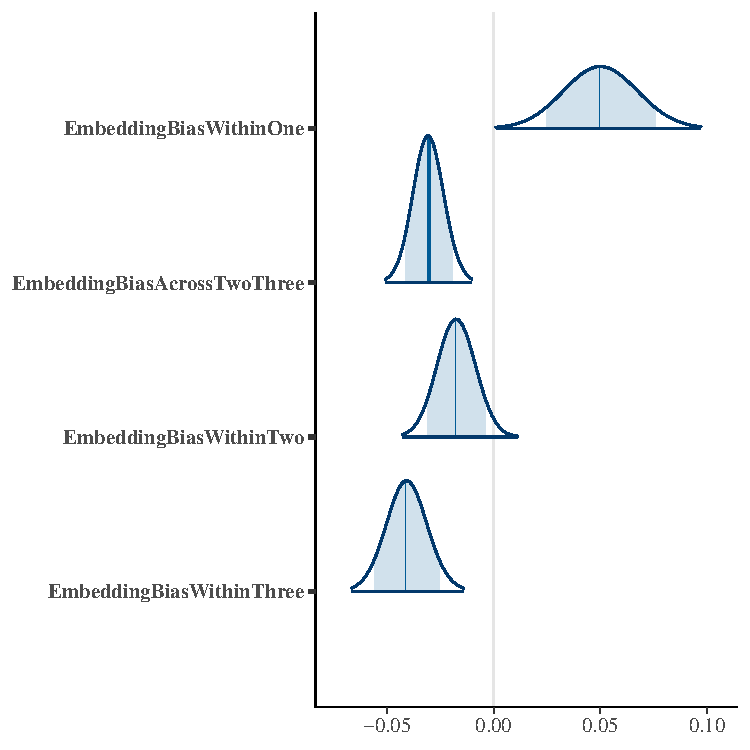
\includegraphics[width=0.3\textwidth]{../resource-rational-surprisal/experiments/maze/meta/controls/figures/posterior-histograms-EmbeddingBias_wikipedia.pdf} &
		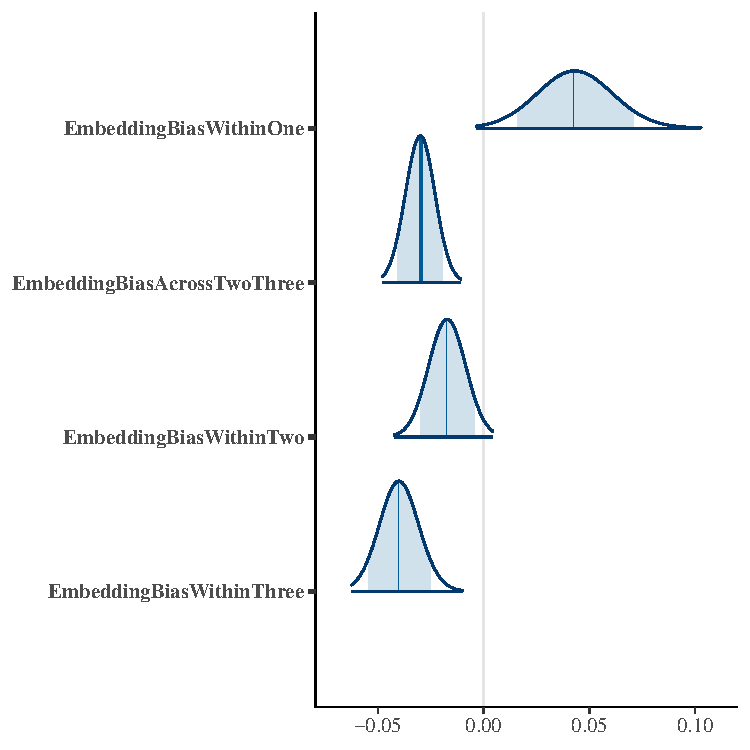
\includegraphics[width=0.3\textwidth]{../resource-rational-surprisal/experiments/maze/meta/controls/figures/posterior-histograms-EmbeddingBias_ukwac.pdf} &
		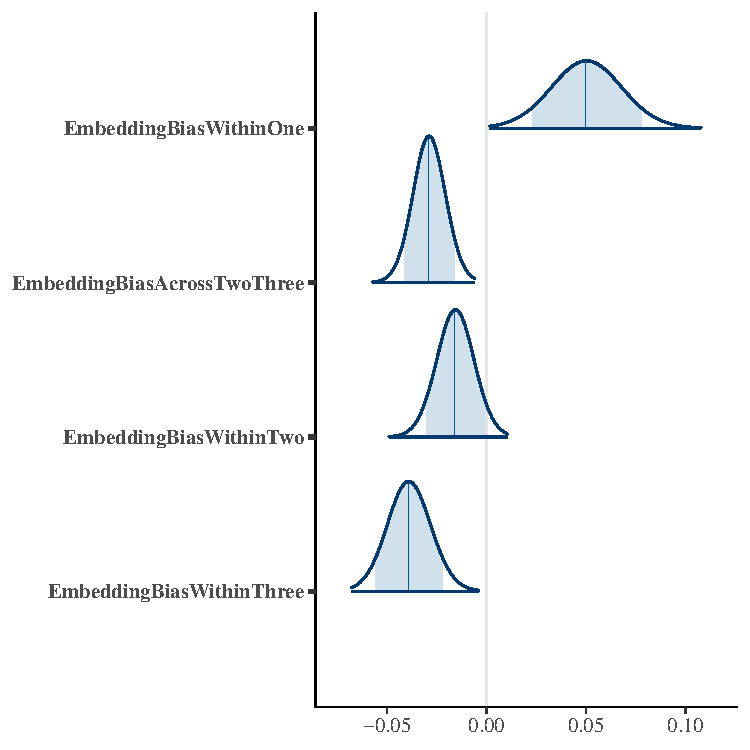
\includegraphics[width=0.3\textwidth]{../resource-rational-surprisal/experiments/maze/meta/controls/figures/posterior-histograms-EmbeddingBias_coca.pdf} &
\end{tabular}
      
	\caption{Posterior of the effect of Embedding Bias on reading times on the final verb (on the data from Section~\ref{sec:meta}), estimating Embedding Bias using three large-scale English corpora.
	The posteriors are obtained from the posterior of the mixed-effects analysis of log-transformed reading times fitted separately using three versions of Embedding Bias; for instance, the effect within \textsc{One} is obtained as $\beta_{EmbeddingBias} -0.9 \beta_{EmbeddingBias:Embedding}$ (cf. Section~\ref{sec:effects-raw-rt}).
	All corpora lead to similar estimated coefficients in the different conditions. This confirms the robustness of the finding to the corpus used for estimating Embedding Bias.}
    \label{fig:posterior-ukwac-coca}
\end{figure}

In Figures~\ref{fig:posterior-ukwac-coca}--\ref{fig:production-posteriors-corpora}, we show that the effect of Embedding Bias found in Experiments 1--3 is robust to different corpora used for estimating Embedding Bias: In addition to Wikipedia, we also considered COCA \cite[][1B words of American English]{Davies2012TheCO} and ukWaC \cite[][2B words primarily of British English]{Ferraresi2008IntroducingAE}.
Results are very similar across the three corpora.
\footnote{In the production study, estimated effects are stronger with ukWaC and COCA counts than with the Wikipedia counts reported in the main paper; this is in part because the word \textit{inkling} is much more common in those corpora than in Wikipedia, leading to different and potentially more reliable estimates of Embedding Bias. We did not include \textit{inkling} in model simulations due to the low number of occurrences in Wikipedia.}


\begin{figure}	
	\begin{tabular}{ccc}
		Wikipedia & ukWaC & COCA \\
		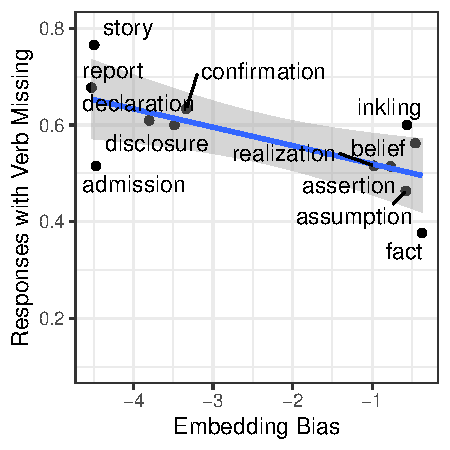
\includegraphics[width=0.3\textwidth]{../resource-rational-surprisal/experiments/production/experiment3_english/Submiterator-master/figures/rates_by_conditional.pdf}&
		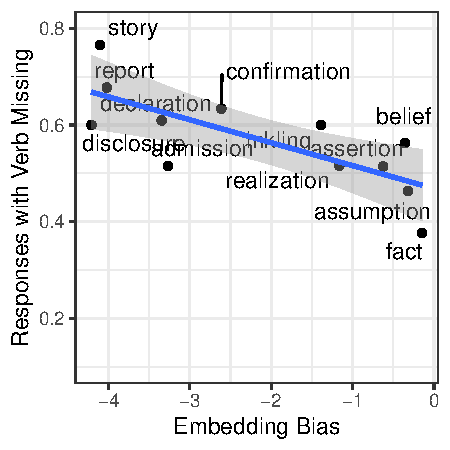
\includegraphics[width=0.3\textwidth]{../resource-rational-surprisal/experiments/production/experiment3_english/Submiterator-master/figures/rates_by_conditional_ukwac.pdf} &
	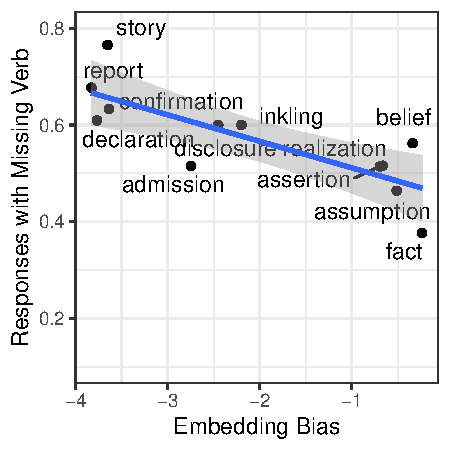
\includegraphics[width=0.3\textwidth]{../resource-rational-surprisal/experiments/production/experiment3_english/Submiterator-master/figures/rates_by_conditional_COCA.pdf}
\\
		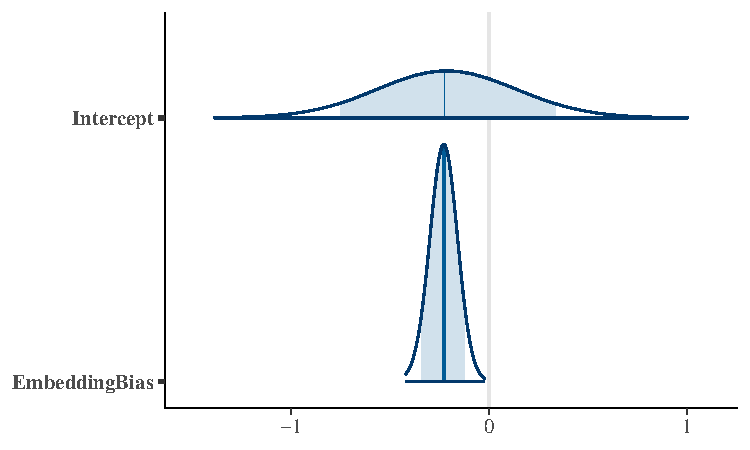
\includegraphics[width=0.3\textwidth]{../resource-rational-surprisal/experiments/production/experiment3_english/Submiterator-master/figures/posterior-histograms.pdf} &
		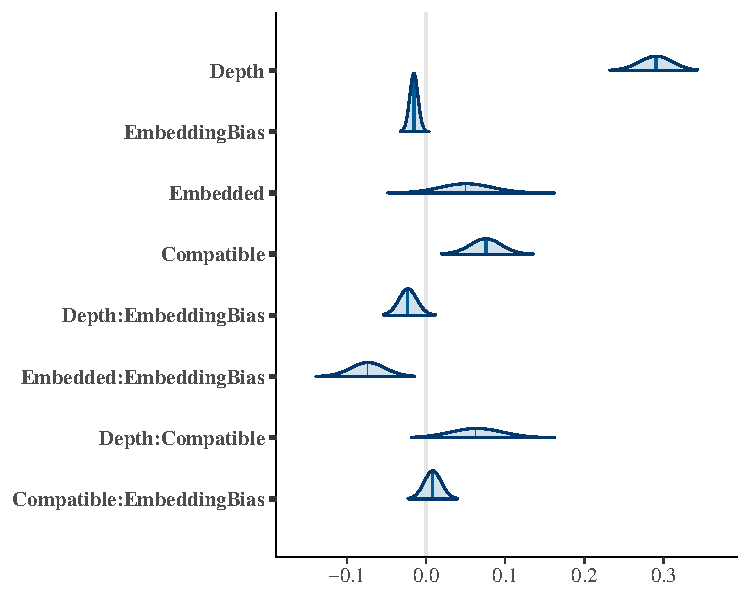
\includegraphics[width=0.3\textwidth]{../resource-rational-surprisal/experiments/production/experiment3_english/Submiterator-master/figures/posterior-histograms_ukwac.pdf}  &
		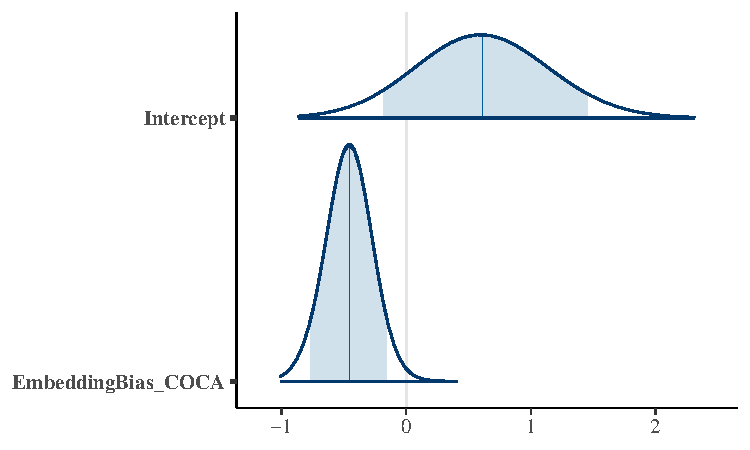
\includegraphics[width=0.3\textwidth]{../resource-rational-surprisal/experiments/production/experiment3_english/Submiterator-master/figures/posterior-histograms_COCA.pdf} \\
		\footnotesize{$\beta=-0.33$, 95\% CrI $[-0.61, -0.06]$}	& \footnotesize{$\beta=-0.40$, 95\% CrI $[-0.70, -0.13]$}  &	\footnotesize{$\beta = -0.46$, 95\% CrI $[-0.77, -0.16]$} \\
		\footnotesize{$P(\beta>0) = 0.01025$} & \footnotesize{$P(\beta>0) = 0.00275$} & \footnotesize{$P(\beta>0) = 0.00375$} \\
	\end{tabular}
	\caption{Results of the English production study when estimating Embedding Bias using Wikipedia (as reported in the main paper) and the two other large corpora described in Section~\ref{sec:embedding-rate-other-corpora}. Top: By-noun rates of incomplete responses. Bottom: Results of mixed-effects analysis (compare Figure~\ref{fig:production-posteriors}). A significant effect of similar effect size is found with all three corpora. }\label{fig:production-posteriors-corpora}
\end{figure}




\subsection{Embedding Bias and other Predictors}

The effect of Embedding Bias consistently observed across experiments in reading times, production, and ratings might be among the more surprising experimental findings in this paper.
In the model, it arises from the differences in posterior probability assigned to the correct number of embedding levels.
Given that this is a new effect not previously reported in the psycholinguistic literature, we asked whether there might be other factors correlated with Embedding Bias that might also capture the observed behavioral data.

We considered the following properties of nouns:
\begin{enumerate}
	\item \textsc{EmbeddingBias}, i.e.

\begin{equation}
		\log P(that|the\ NOUN)
\end{equation}
		estimated on the corpora discussed in Section~\ref{sec:embedding-rate-other-corpora} (Wikipedia, ukWaC, COCA).

		Note that \textsc{EmbeddingBias} is the difference  of (2) and (3) listed below.

	\item \textsc{MarginalProbability}:

\begin{equation}
		\log P(the\ NOUN)
\end{equation}



\item \textsc{JointProbability}:

\begin{equation}
		\log P(the\ NOUN\ that)
\end{equation}



\item \textsc{ComplementClauseBias}: the log-probability that a noun, when it is followed by \textit{that} embeds a complement clause rather than a relative clause:
\begin{equation}
		\log P(SC|the\ NOUN\ that)
\end{equation}
This probability is referred to as \emph{inclusive CC noun bias} by \citet{Staub2018RelativeCA}.


Estimating this term requires syntactic analysis distinguishing SCs from other constructions (e.g., relative clauses).
We found that automatic parsing was not fully reliable in distinguishing these; thus, we followed \citet{Staub2018RelativeCA} in using manual annotation.
While they used search engine results, we found those (as obtained in 2021) strongly biased towards names and website titles.
We thus instead sampled occurrences of ``the NOUN that'' from the English Wikipedia (the same corpus used to estimate the other probabilities).
A trained linguist annotated these for (1) SC, (2) RC (``The fact that was mentioned...''), (3) Other (``The part of the report that was written first...'') readings.
Annotation continued until either a Binomial confidence interval for $log P(SC|\text{the NOUN that})$ had width $\leq 0.15$, or no further data was availbale.
We conducted annotation for 95 nouns from the initial pool (see Section~\ref{sec:nouns}), a superset of the nouns considered in the experiments and simulations.

For all relevant nouns, this condition was reached after annotating less than 200 samples.
		Results are deposited in the project repository.\footnote{\url{https://gitlab.com/m-hahn/resource-rational-surprisal/-/blob/main/materials/nouns/corpus_counts/wikipedia/RC_annotate/results/collectResults.py.tsv}}.

Across the 95 nouns, we found that $P(SC|\text{the NOUN that})$ was generally close to $1$ (mean 0.88; median 0.97; minimum 0.2 for `relief' and `bet'; these are not used in the experiments). 



\item \textsc{SubjectBias}: the log-probability that a noun is a subject.
	Here, we found automatic parsing to be sufficiently reliable.
		We parsed about 20\% of the English Wikipedia using Stanza~\citep{Qi2020StanzaAP} and recorded the fraction of times a noun's dependency label was \textit{nsubj} or a subtype.

		We reasoned that, under accounts of center embeddings in theories of cue-based retrieval (see Section~\ref{sec:other-theories}), \textsc{SubjectBias} rather than \textsc{EmbeddingBias} could determine how likely humans might be to (erroneously) attach a noun such as \textit{report} as the subject of \textit{annoyed} in \textit{The report that the doctor annoyed the patient...}, causing difficulty on the final verb.

	\item \textsc{WordLength} measured in characters

	\item \textsc{Entailing}: entailing/non-entailing contrast, see Section~\ref{sec:nouns}

	\item \textsc{HomophoneVerb}: homophony with a verb (e.g., remark, report)
	
	\item \textsc{Deverbal}: derivational relationship with a verb, including homophony (e.g., information)
\end{enumerate}

We first fitted, for each of these predictors, a frequentist mixed-effects model with lme4~\citep{Bates2014FittingLM} (using ML, not REML), and computed its log-likelihood. 
These models were fitted on the subset in the \textsc{Two}/\textsc{Three} conditions of the data used in Section~\ref{sec:meta}, and included \textsc{Two}/\textsc{Three} contrast and the \textsc{Compatibility} contrast, their interaction, and the additional predictor of interest.
Due to convergence issues, the model included only random intercepts.
The log-likelihood values for each predictor are shown in Figure~\ref{fig:predictors-aic}.
\textsc{EmbeddingBias} estimated from the three corpora result in the best model fits (lowest negative log-likelihood), with some distance to the other predictors.
Interestingly, the ukWaC version provided the best model fit; this might be either due to genre differences or the presence of British English speakers among the participant population on Prolific.

We further used forward model selection with BIC to determine whether better fit can be obtained by combining different predictors.
This was not the case, as the best model overall included only \textsc{EmbeddingBias}. 

In conclusion, Embedding Bias is a much better predictor of noun-specific reading times on the final verb in the \textsc{Two}/\textsc{Three} condition than the other predictors investigated.
There is also little evidence that adding any further predictor to it would improve model fit.

\begin{figure}
	\centering
    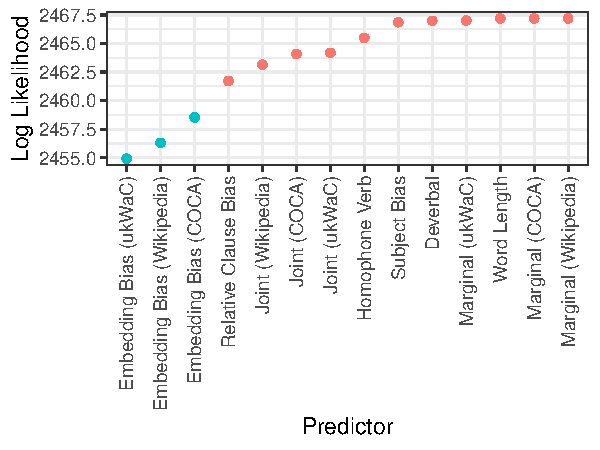
\includegraphics[width=0.5\textwidth]{../resource-rational-surprisal/experiments/maze/meta/controls/analyze_Previous_AIC_Single_R.pdf}


	\caption{Negative log-likelihoods (lower is better) of models of reading times with various properties of nouns added. The best model fit is achieved by Embedding Bias (blue), as estimated on three large corpora of English.}\label{fig:predictors-aic}
\end{figure}


As a further way of understanding how Embedding Bias predicts reading times, we conducted the following procedure.
We fitted a version of the mixed-effects model with all fixed and random effects involving Embedding Bias removed.
This means that any by-noun variation is now encoded in the fitted random effects.
For each noun, its effect on reading times in the \textsc{Two} and \textsc{Three} conditions is given as its random intercept plus 0.1 times its random slope for the \textsc{Embedded} fixed effect.
This provides a measure of the noun's impact on reading times, without any bias towards an effect of Embedding Bias or any property of nouns.
In Figure~\ref{fig:effect-embrate-corr}, we plot the posterior means for these effects against Embedding Bias. 
We found a strong correlation between the two measures ($R = -0.72$, $p=1.5\cdot 10^{-7}$; $\rho = -0.70$, $p=1.3 \cdot 10^{-6}$).
\footnote{We also computed the correlation across different posterior samples, instead of for the mean. We obtained a mean correlation of $R=-0.59$, $95\%$ CrI $[-0.72, -0.45]$.}



In conclusion, Embedding Bias is not just a better predictor of reading times on the final verb than other properties of nouns, but also accounts for a substantial amount of variance in the by-nouns effect on reading times.

An interesting connection can be made to work suggesting a role of mutual information in language and human language processing \citep[e.g.][]{Culbertson2020FROMTW}:
Up to a constant, Embedding Bias is equal to the mutual information between the noun and \textit{that}.
In this sense, anticipating the final verb is easier when the mutual information between the noun and the crucial functional element (the word \textit{that}) is higher.



\begin{figure}
	\centering
    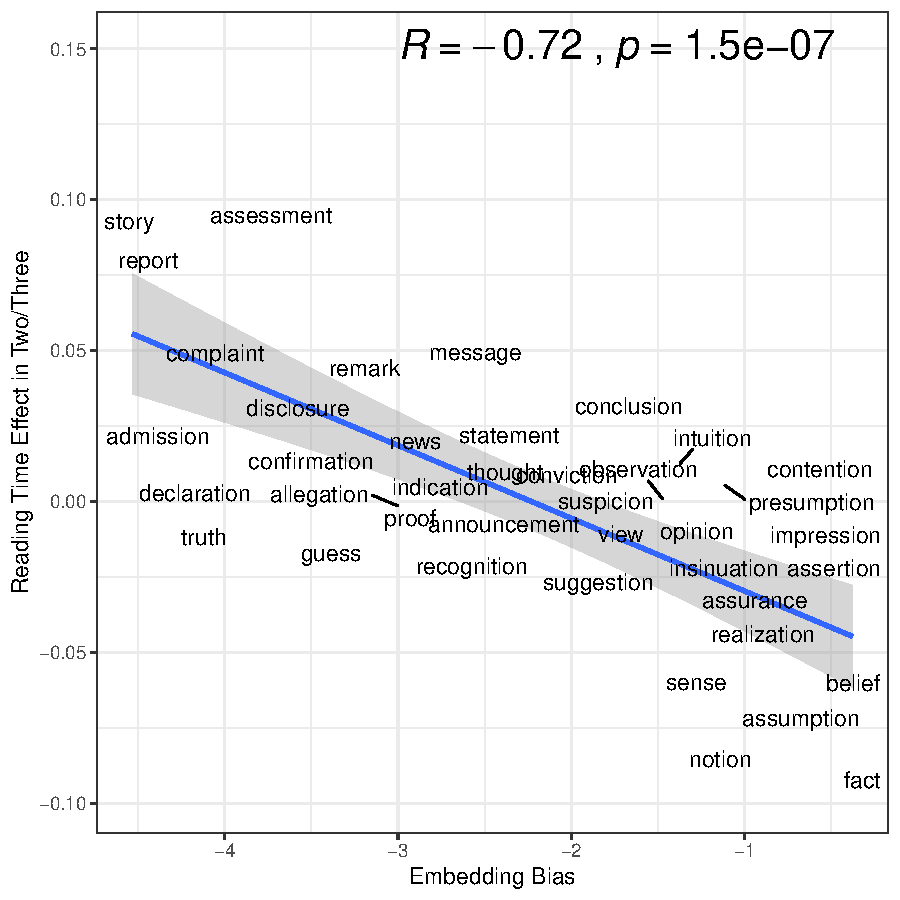
\includegraphics[width=0.6\textwidth]{../resource-rational-surprisal/experiments/maze/meta/output/plotNounIntercepts_R.pdf}


	\caption{Comparing relative reading time effects of nouns in the \textsc{Two}/\textsc{Three} conditions with Embedding Bias as estimated from Wikipedia. Reading time effects were estimated using a mixed-effects analysis of reading times on the critical verb, but in which fixed effects including embedding bias were removed (see text for details). A strong correlation between the two confirms that reading time differences on the critical verb closely track embedding bias.}\label{fig:effect-embrate-corr}
\end{figure}



